% Ubah judul dan label berikut sesuai dengan yang diinginkan.
\section{DESIGN AND SYSTEM IMPLEMENTATION}
\label{sec:desainimplementasi}

% Ubah paragraf-paragraf pada bagian ini sesuai dengan yang diinginkan.
This research is an application in the field of \textit{Natural Language Processing} by using \textit{Deep Learning} in order to detect emotions/\textit{Emotion} from social media texts obtained from \textit{Twitter} automatically. In the data training process, data is obtained from the source \textit{Emotion Classification on Indonesian Twitter Dataset} \cite{dataset} containing 4401 \textit{tweet} which have been labeled with 5 emotions, namely \textit{love}, \textit{anger }, \textit{sadness}, \textit{joy}, \textit{fear}. The personal data in the \textit{Dataset} has been cleaned, for example, the \textit{username} of each user has been replaced with the word \textit{[USERNAME]}, the related link has been replaced with \textit{[URL]}, and \textit{Sensitive Number} has been replaced with \textit{[SENSITIVE-NO]}.

\subsection{Data Acquisition}

In the data acquisition stage, the data is taken from the \textit{dataset} that has been created. Inside it is labeled which will later be classified using the \textbf{BERT} method. The related \textit{Dataset} contains 4401 \textit{tweet} in Indonesian which has 5 labels \textit{emotion}, namely \textit{love}, \textit{anger}, \textit{sadness}, \textit {joy}, \textit{fear}. For now, the entire \textit{dataset} can be accessed and downloaded at the link \url{https://github.com/meisaputri21/Indonesian-Twitter-Emotion-Dataset} and related publications can be accessed via the link \url{https:/ /www.researchgate.net/publication/330674171_Emotion_Classification_on_Indonesian_Twitter_Dataset}. The division of each number of \textit{Tweet} in each \textit{Emotion} is as follows:

\begin{figure}[h!]
  \begin{center}
    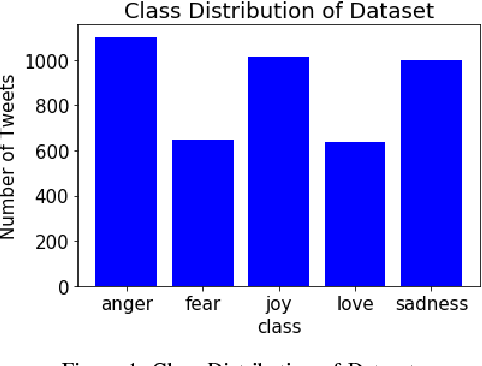
\includegraphics[width= \linewidth]{template-paper-ieee-main/gambar/pembagian_dataset.png}
    \caption{The Division of each \textit{Emotion} in the Dataset}
    \label{fig: dataset}
  \end{center}
\end{figure}

\begin{figure}[h!]
  \begin{center}
    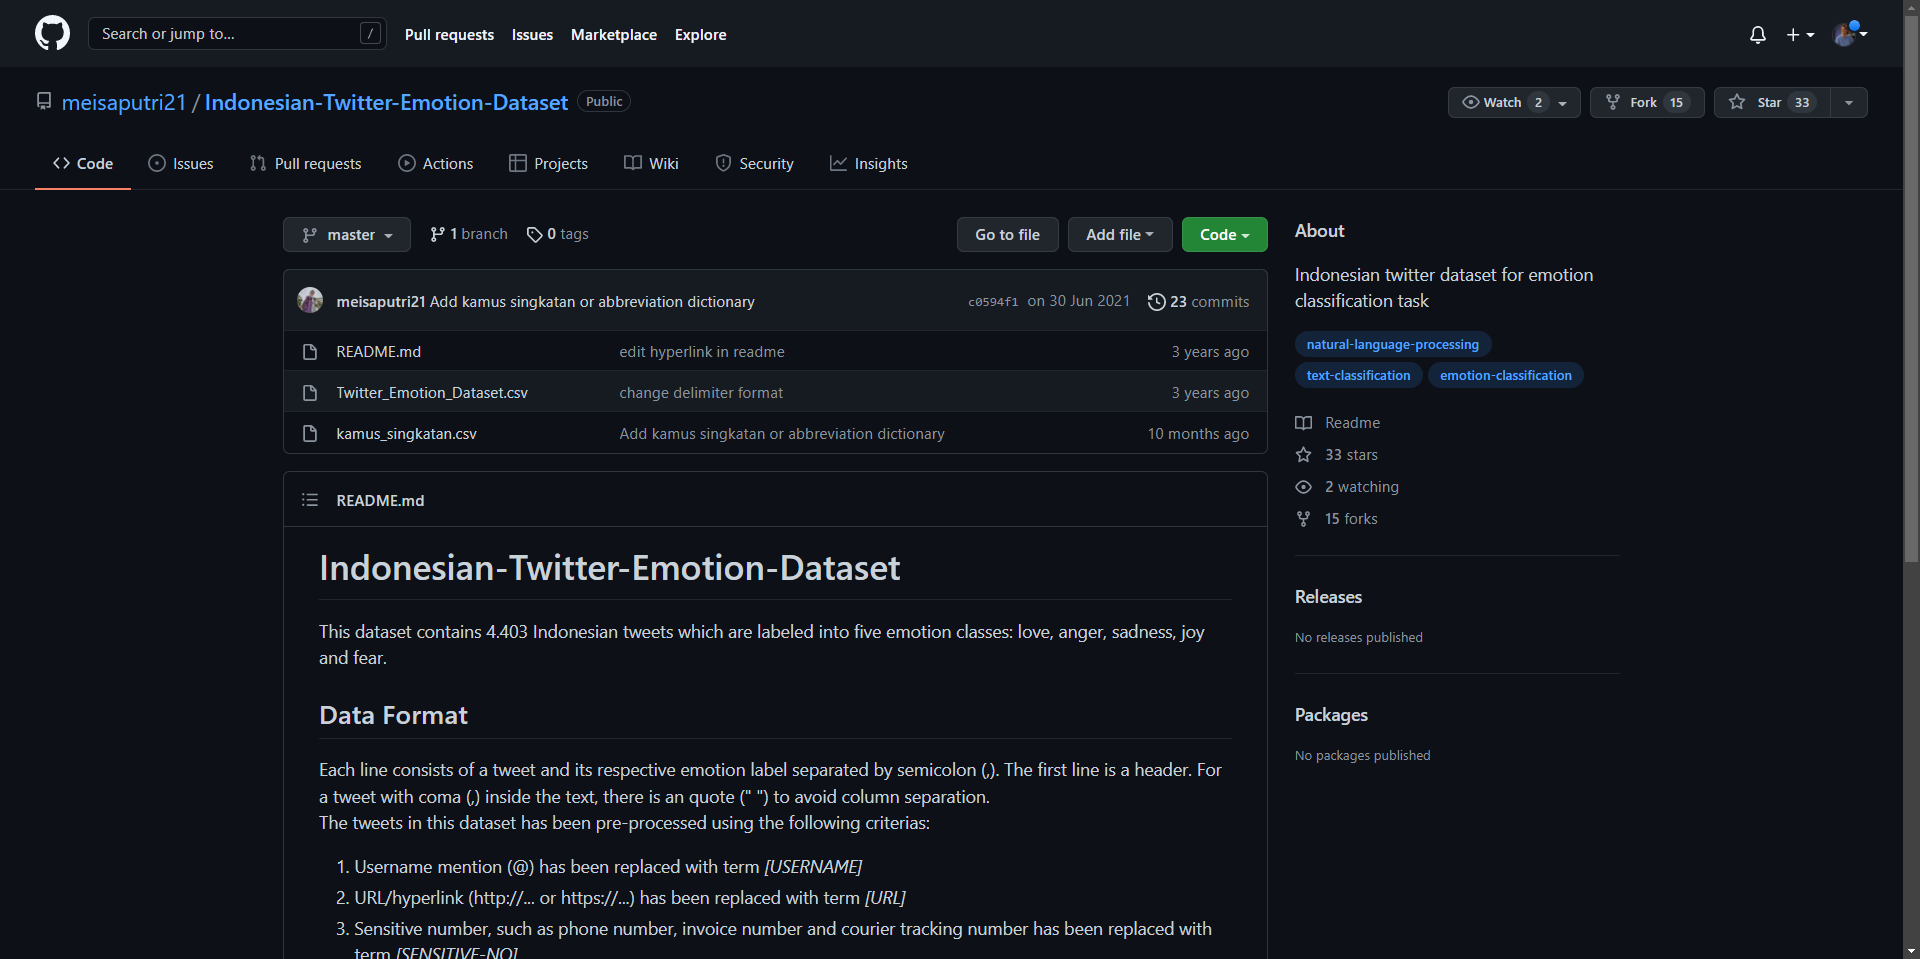
\includegraphics[width= \linewidth]{template-paper-ieee-main/gambar/01_dataset.png}
    \caption{Retrieved source \textit{Dataset}}
    \label{fig: dataset}
  \end{center}
\end{figure}

\begin{figure}[h!]
  \begin{center}
    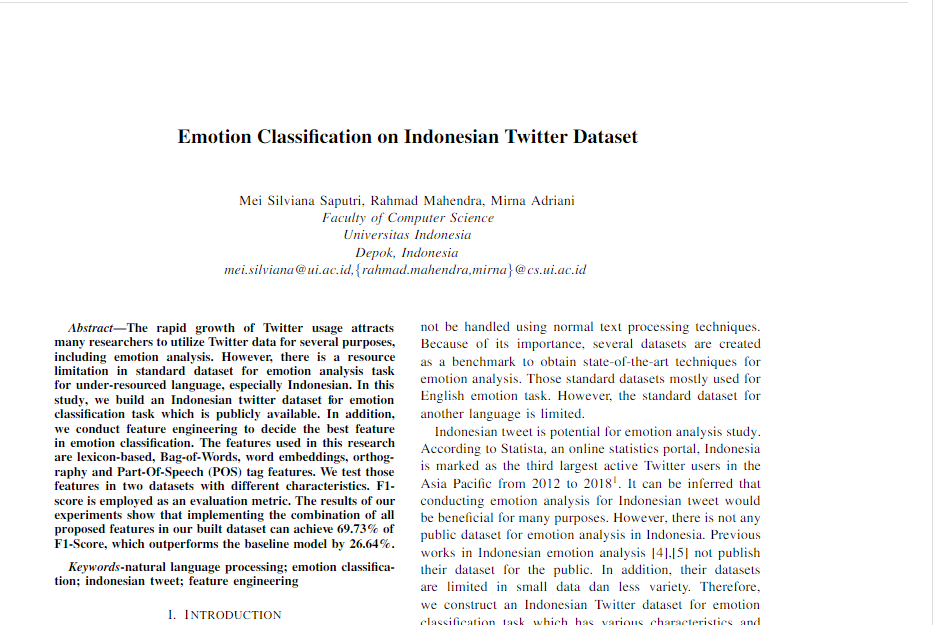
\includegraphics[width= \linewidth]{template-paper-ieee-main/gambar/02_publikasi.png}
    \caption{Publication Source of retrieved \textit{Dataset}}
    \label{fig: publikasi}
  \end{center}
\end{figure}

\subsection{\textit{Preprocessing}}

\begin{figure}[]
  \begin{center}
    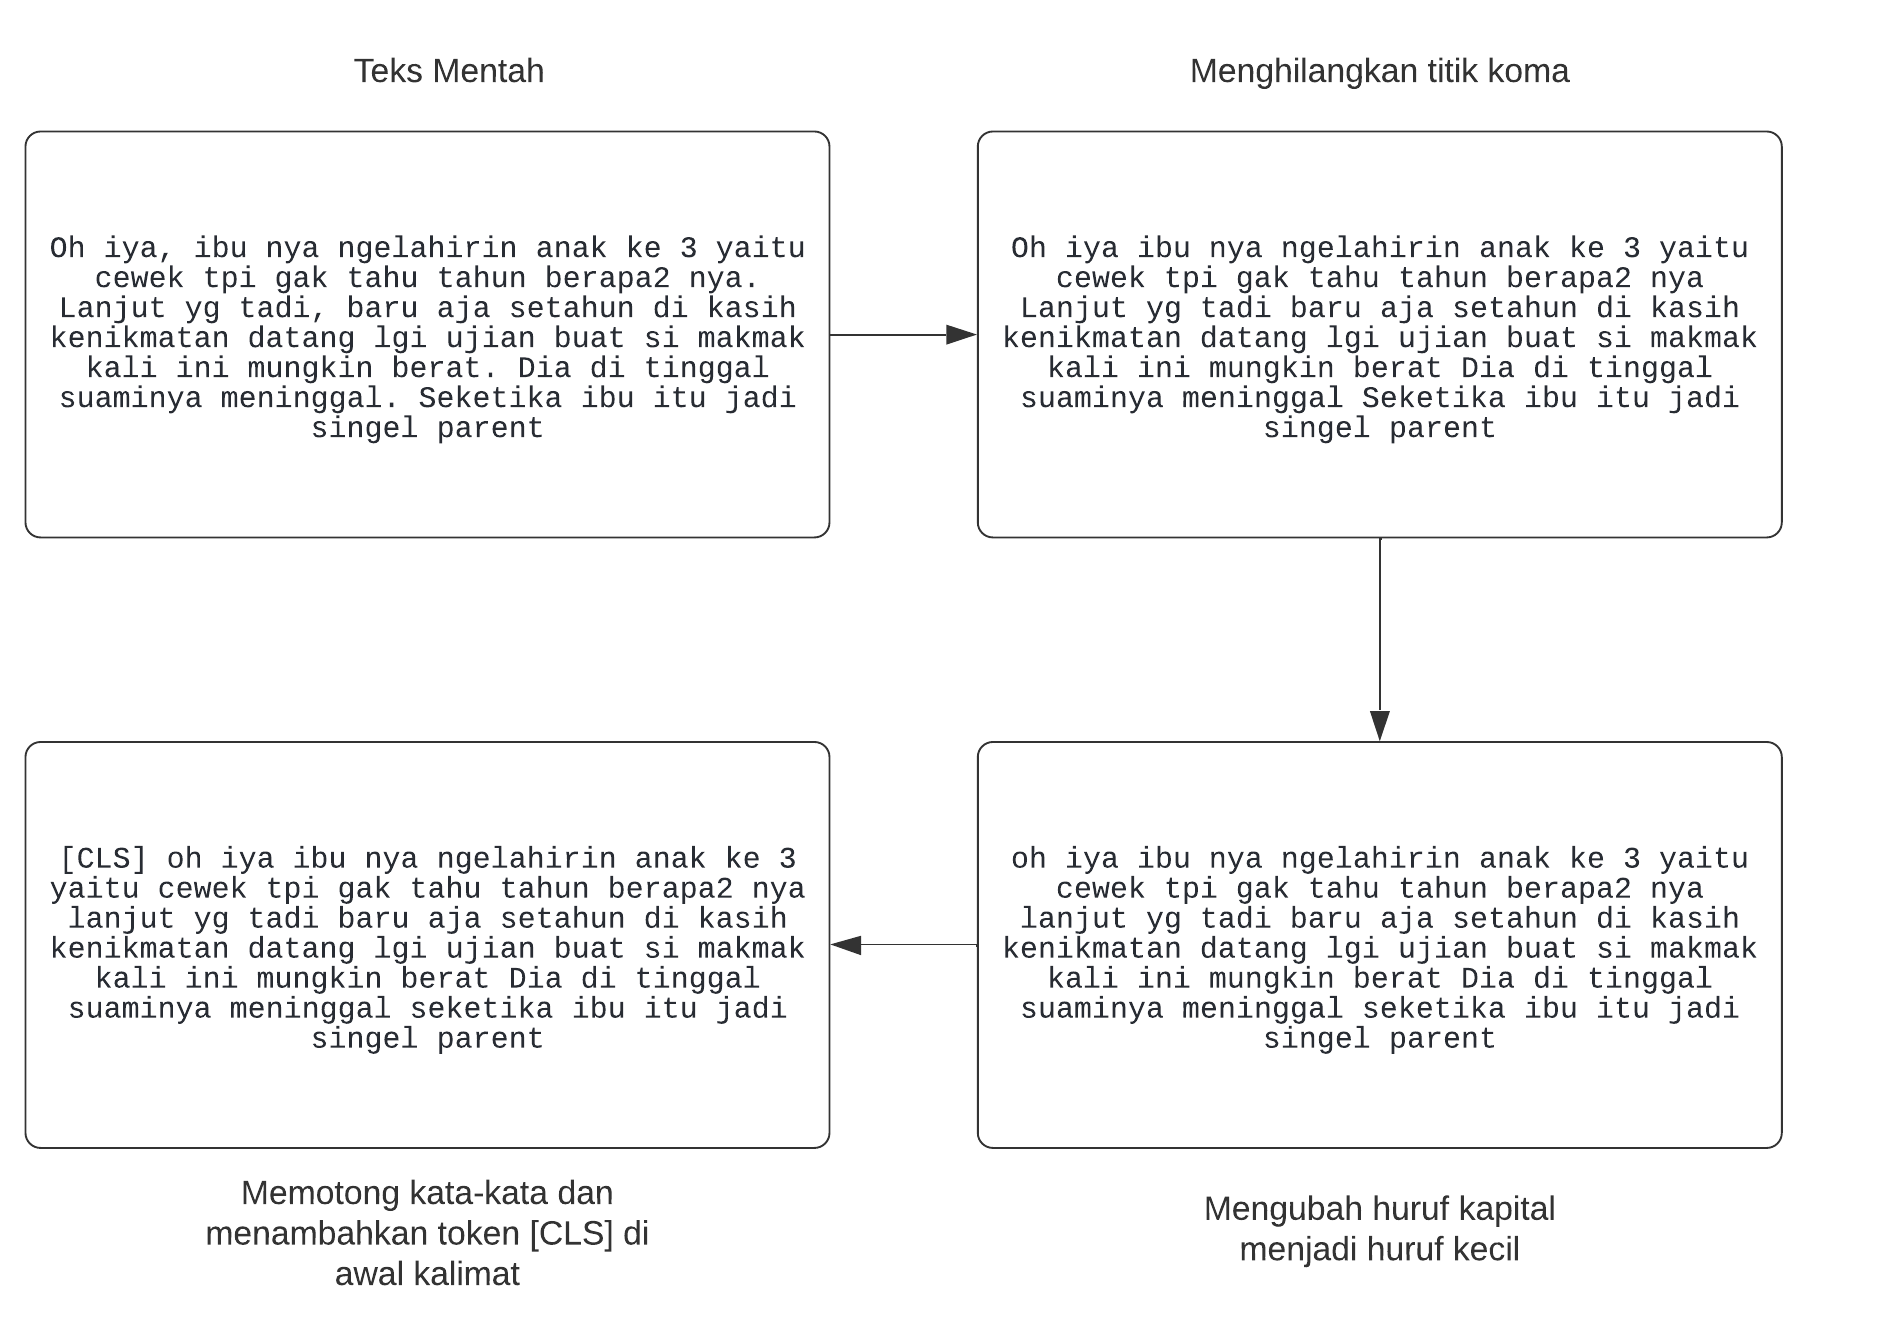
\includegraphics[width= \linewidth]{template-paper-ieee-main/gambar/08_nonstemming.png}
    \caption{Preprocessing method with type \textit{non-stemming}}
    \label{fig: metodologi_preprocessing_nonstemming}
  \end{center}
\end{figure}

In the \textit{Preprocessing} process, the data will be cleaned before the data is processed using the \textbf{BERT} model. There are two methods \textit{Preprocessing} that divide into two types \textit{Dataset}. Besides wanting to test the performance of the model on \textbf{BERT}, the reason the \textit{Preprocessing} method is divided into two is to find out whether the process of changing the basic structure of a sentence changes the accuracy of the model or not. The first method is to use the \textit{non-stemming} method, which is depicted in the image \ref{fig: methodology_preprocessing_nonstemming}. In this section, the contents of each \textit{Feature} in \textit{Dataset} will be changed several parts, but do not remove the meaning/value of the contents. The \textit{Preprocessing} process includes removing periods and commas and changing the capital letters contained in each text.

\begin{figure}[]
  \begin{center}
    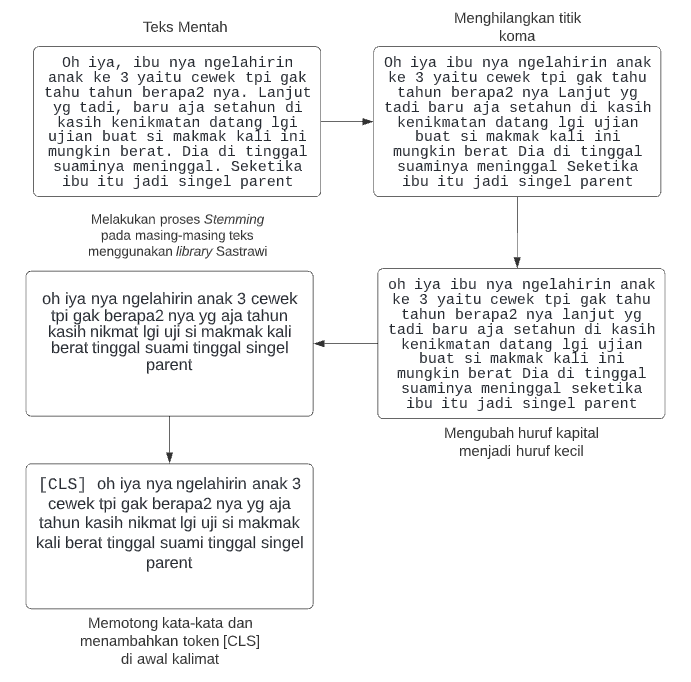
\includegraphics[width= \linewidth]{template-paper-ieee-main/gambar/09_stemming.png}
    \caption{Preprocessing method with type \textit{stemming}}
    \label{fig: metodologi_preprocessing_stemming}
  \end{center}
\end{figure}

Then the second method depicted in the image is the \textit{Stemming} process. \textit{Stemming} is a method to reduce inflectional/affixed words in a language to their basic form (\textit{stem}). In this process, we use \textit{Library} named \textbf{Sastrawi} which reduces the inflected words in Indonesian so that they can become sentences according to the basic form/close to the standard form. The process of the \textit{Stemming} method is actually the same as the \textit{non-stemming} method, starting with removing the semicolon, then changing the capital letters to lowercase letters. However, before adding the \textbf{[CLS]} token, the text will be processed using \textbf{Literary} to be converted into text with the basic form. The \textit{Stemming} process ends by adding the \textbf{[CLS} token at the beginning of the sentence.

BERT has a maximum of 512 words or tokens that can be processed at one time, so text abbreviations must be shortened by taking the first 280 characters (according to the maximum number of characters when the user \textit{Twitter} sends one \textit{ Tweet}), the last or a combination of the two forms. Chisun et al. found that retrieving text by taking the first 128 words in the middle and retrieving 382 words at the end resulted in better accuracy in some tasks \cite{sun2019fine}.

In addition, the dataset will also be divided which initially amounted to 4401 which will be divided into 3 parts with the provisions that 70\% will be used during the \textit{training} process, 10\% will be used for the validation process, and the remaining 20\% will be used at the time of testing.

For more details, please see the \ref{tab:dataset_section} table. From the table it can be seen that the division and total of the dataset are appropriate.

\begin{table}[]
    \caption{Dataset Sharing Details}
    \label{tab:dataset_section}
    \centering
    \begin{tabular}{ | l | l | l | l | l | l | l | }
        \hline
        \textbf{Bagian}                      & \textbf{Anger} & \textbf{Fear} & \textbf{Happy} & \textbf{Love} & \textbf{Sadness} & \textbf{Total Data} \\ \hline
        \textit{Training}                    & 760            & 466            & 719          & 445              & 690                  & 3080        \\ \hline
        \textit{Validasi}                    & 139            &  34           & 93          & 73              &   102               &  441       \\ \hline
        \textit{Pengujian}                    & 202            & 149            & 205          & 119               & 205                  & 880        \\ \hline
        \multicolumn{6}{|l|}{\textbf{Total}} & \textbf{4401}                                         \\ \hline
    \end{tabular}
\end{table}


\subsection{Training Process}

\begin{figure}[h!]
  \begin{center}
    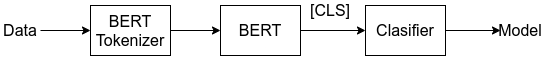
\includegraphics[width= 0.9\linewidth]{template-paper-ieee-main/gambar/training.png}
    \caption{Training Method}
    \label{fig: metodologi_training}
  \end{center}
\end{figure}

At this stage, first the \textit{Preprocessing} process will be carried out by \textbf{BERT Tokenizer}. This tokenizer is a process in which a word in a sentence becomes a token according to the \textit{Word Embedding} provided by BERT. After that, the BERT Model will train the data from the \textit{Preprocessing} Tokenizer from the \textit{Word Embedding}. The \textit{Output} of the BERT Model is the \textbf{[CLS]} token which will be entered into the text. This token will be entered into the classification algorithm to determine between \textit{Feature} and its \textit{Target}. The image \ref{fig: methodology_training} can be used as an explanation.

At the \textit{Training} stage, adjustments were also made to settings such as \textit{Batch}, \textit{Learning Rate}, \textit{Epoch}, \textit{Hidden Dropout}, and \textit{Epsilon}. \textit{Batch} or \textit{batch size} is \textit{hyperparameter} which specifies the number of samples to be worked on before updating the internal model parameters. \textit{Batch} in this case iterates over one or more samples and makes predictions.

The \ref{fig: hyperparameter} table is further information on the \textit{Hyperparameter} value used in this study.


\begin{table}[!h]
  \caption{BERT Configuration}
  \label{tab:bert_config}
  \centering
  \begin{tabular}{ | l | l | }
    \hline
    \textbf{Jenis Konfigurasi} & \textbf{Keterangan} \\ \hline
        \textit{\textbf{epoch}}          & 3                              \\ \hline
        \textit{\textbf{batch size}}     & 8                              \\ \hline 
        \textit{\textbf{learning rate}} & 2e-5                           \\ \hline
        \textit{\textbf{hidden dropout}} & 0.1                   \\ \hline 
        \textit{\textbf{epsilon}}        & 1e-4 dan 1e-8                          \\ \hline
  \end{tabular}
  \label{fig: hyperparameter}
\end{table}

\subsection{Testing Method}

The testing process in this study is divided into 2 parts, the first part is carried out when the model has finished doing the \textit{training} process but still has an unfinished \textit{epoch} iteration. This process is called validation. The next part of the testing process is to do \textit{test}. Just like during the validation process, the dataset used is completely different from the data used at the time of \textit{training} and at the time of \textit{validation}. From this process, it can be concluded whether a model can be improved again by means of \textit{re-training} and changing some parameters and configurations that have been set during the \textit{training} process, or whether the model is considered good enough and will continue to the next process.

\subsection{Performance Analysis}

After carrying out the testing process, the Performance Analysis process is carried out. In this process, a calculation is made of how well the performance of the model that has been tested is calculated. Calculations in the Performance Analysis process use several references called \textit{Metrics}. \textit{Metrics} used is \textit{Metrics} which is used for classification algorithms such as \textit{Confusion Matrix}, \textit{Accuracy Score}, \textit{Precision}, \textit{Recall}, and \textit{F1 Score}. The set of \textit{Metrics} can be calculated in one iteration using a feature named \textit{Classification Report}.